\documentclass[a4paper,twoside]{article}

\usepackage{epsfig}
\usepackage{subcaption}
\usepackage{calc}
\usepackage{amssymb}
\usepackage{amstext}
\usepackage{amsmath}
\usepackage{amsthm}
\usepackage{multicol}
\usepackage{pslatex}
\usepackage{algorithm2e}
\usepackage[bottom]{footmisc}
\usepackage{SCITEPRESS}
\usepackage{cite}
\usepackage{hyperref}
\usepackage[none]{hyphenat}
\usepackage[table]{xcolor}
\definecolor{pastelorange}{HTML}{F5D08A}
\begin{document}

\title{Efficient Multi-Temporal Building Change Detection with Reduced-Rank Linear Attention}

\author{\authorname{Ricardo A. Acuña-Villogas\sup{1}\orcidAuthor{0009-0005-7543-2232}, Germain García-Zanabria\sup{4}\orcidAuthor{0000-0003-3266-9043}, Cristian Lopez\sup{3}\orcidAuthor{0000-0002-2568-650X} and Rensso Mora-Colque\sup{2}\orcidAuthor{0000-0003-4734-8752}}
\affiliation{\sup{1}\sup{2}\sup{3}\sup{4}Department of Data Science, University of Engineering and Technology, Barranco, Lima, Peru}
\email{\{ricardo.acuna,  ggarciaz, clopezd, rmora\}@utec.edu.pe}
}

\keywords{Building Change Detection, Linear Attention, Remote Sensing, Computational Efficiency, Satellite Imagery}

\abstract{
Transformer-based architectures have become the dominant paradigm for bi-temporal building change detection (BCD). However, their application to very high–resolution (VHR) imagery remains limited by the quadratic complexity of multi-head self-attention (MHSA). This work introduces RALA-ChangeFormer, an efficient variant of ChangeFormer that replaces the encoder’s MHSA modules with rank-augmented linear attention (RALA). The integration preserves the hierarchical structure of the original model and maintains its ability to perform bi-temporal spatio–temporal reasoning. Experiments on the LEVIR-CD and DSIFN-CD benchmarks show that RALA-ChangeFormer delivers segmentation accuracy comparable to the baseline, with variations within standard training variance. The method reduces attention-related GFLOPs, lowers peak GPU memory consumption, and enables substantially larger batch sizes at multiple resolutions. Ablation studies confirm that the efficiency gains arise primarily from the encoder, where token counts are highest. Overall, the results demonstrate that rank-augmented linear attention provides a practical accuracy–efficiency trade-off for VHR BCD. The proposed approach improves computational scalability without sacrificing predictive performance, making high-resolution or large-scale training more accessible under fixed hardware constraints.
}

\onecolumn \maketitle \normalsize \setcounter{footnote}{0} \vfill

\section{\uppercase{Introduction}}
\label{sec:introduction}

Multi-temporal Building Change Detection (BCD) from very high–resolution (VHR) satellite imagery plays a crucial role in urban expansion monitoring, infrastructure management, and post–disaster assessment \cite{Daudt2018SiamICIP,Zhang2020FusionNet,Hussain2013Review}. Given two or more images of the same geographic area acquired at different times, the goal is to determine whether individual buildings have been newly constructed, removed, or altered in their footprint or roof structure. The task is typically formulated as a bi-temporal semantic segmentation problem \cite{Zhang2020Survey,Shafique2022Review}, where a model predicts a binary change mask from paired inputs. Public benchmarks such as LEVIR-CD \cite{Zheng2020LEVIR} and DSIFN-CD \cite{Shen2021DSIFN} have been instrumental in advancing BCD because they offer sufficiently large, diverse, and well-annotated bi-temporal samples to train and reliably evaluate deep models on building-scale structural changes. Fundamentally, accurately predicting change regions requires a dual capability, the model must: (i) resolve subtle, fine–grained alterations at the building level, and (ii) integrate broader spatial–temporal context to disambiguate true structural changes from irrelevant variations such as illumination or seasonal effects. In this context, RALA-ChangeFormer \cite{Fan2025RALA} satisfies the dual requirement while substantially reducing computational cost in comparison to the baseline ChangeFormer \cite{Bandara2022ChangeFormer}. Table~\ref{tab:intro_teaser} shows a comparison of RALA-ChangeFormer and ChangeFormer with different datasets.

\begin{table}[t]
\centering
\caption{Comparison between ChangeFormer (CF) and the proposed RALA-ChangeFormer (RALA-CF) on two benchmarks with input dimension 256 x 256 and batch 16.}
\label{tab:intro_teaser}
\resizebox{\columnwidth}{!}{
        \begin{tabular}{lcc}
        \hline
        \textbf{Dataset} & \textbf{ChangeFormer} & \textbf{RALA-CF} \\
        \hline
        \multicolumn{3}{l}{\textbf{LEVIR-CD \cite{Zheng2020LEVIR}}} \\[2pt]
        F1          & 90.40  & 89.87 \\
        IoU         & 82.48  & 81.60 \\
        FLOPs (G)   & 138.77 & \textbf{135.62} \\
        \hline
        \multicolumn{3}{l}{\textbf{DSIFN-CD \cite{Shen2021DSIFN}}} \\[2pt]
        F1          & 86.67  & 84.07 \\
        IoU         & 76.48  & 73.96 \\
        FLOPs (G)   & 248.77 & \textbf{228.62} \\
        \hline
        \end{tabular}
}
\end{table}

In the same vein, motivated by the challenges inherent to bi-temporal semantic segmentation, recent years have witnessed a shift from convolutional Siamese architectures to Transformer-based models for BCD. Methods such as BIT \cite{Chen2022BIT}, SNUNet \cite{Fang2021SNUNetCD} and ChangeFormer \cite{Bandara2022ChangeFormer} leverage self-attention to capture long-range dependencies and global spatial–temporal context, achieving state-of-the-art performance on multiple datasets. Vision Transformer (ViT) architectures \cite{Dosovitskiy2021ViT,Raghu2023RevengeViT, Fan2024ViTAR} have demonstrated strong representational capacity and scalability in large-scale visual recognition tasks. Their ability to model non-local interactions makes them naturally attractive for multi-temporal reasoning. However, these advantages come with a significant computational burden. Standard self-attention requires quadratic complexity $\mathcal{O}(N^2)$ in both time and memory, considering $N$ as the number of tokens in the input. In multi-temporal BCD, each sample contains two high-resolution images, effectively doubling the sequence length and further amplifying the quadratic cost. As a result, existing Transformer-based approaches often rely on small patch sizes, heavy downsampling, or prohibitively small batch sizes, limiting their scalability and slowing experimentation in practical settings.

To alleviate this bottleneck, a wide range of \emph{efficient attention} mechanisms—kernelized linear attention \cite{Katharopoulos2020Linear,Choromanski2021Performer}, low-rank approximations \cite{Wang2020Linformer,Xiong2021Nystromformer}, and sparse or windowed attention widely used in vision \cite{Liu2021Swin,Wei2023Sparsifiner}—have been proposed to reduce complexity to near-linear in $N$. Despite their theoretical appeal, these methods often suffer from a critical issue: \emph{linear attention inherently collapses the rank of the key–value (KV) representation}, drastically reducing feature diversity and degrading accuracy in dense prediction tasks, especially in vision. Recent studies formalize this phenomenon and introduce the RALA \cite{Fan2025RALA} formulation to mitigate it by explicitly increasing the rank of the intermediate representations through learned token-wise weighting and output modulation. RALA breaks the traditional low-rank/accuracy trade-off observed in earlier linear attention variants.

Although RALA has demonstrated strong performance in natural image classification and general vision benchmarks \cite{Fan2025RALA}, its applicability to multi-temporal semantic segmentation remains unexplored. In particular, it is unknown whether the rank-preserving properties of RALA translate effectively to bi-temporal encoder–decoder architectures such as ChangeFormer, where accurate BCD requires both fine-grained local discrimination and global spatio–temporal reasoning. This gap is especially relevant given the computational constraints of VHR remote sensing, where efficient attention mechanisms must reduce complexity without degrading segmentation accuracy.

In this work, the gap is addressed by introducing \textbf{RALA-ChangeFormer}, an efficient variant of ChangeFormer in which each Transformer block replaces quadratic self-attention with the RALA mechanism, a rank-augmented linear attention formulation that expands the key–value space through a weighted mixture of multiple low-rank projections, preventing the collapse typically observed in standard linear attention. The goal is to reduce the computational and memory cost of multi-temporal BCD while preserving segmentation accuracy. The analysis examines how rank augmentation behaves within the hierarchical encoder–decoder design of ChangeFormer and quantifies its impact on performance, FLOPs, GPU memory consumption, and maximum feasible batch size.

The main contributions of this work are:
\begin{itemize}
    \item The introduction of \textbf{RALA-ChangeFormer}, a rank-augmented linear attention variant of ChangeFormer that achieves near-linear complexity while maintaining competitive accuracy in urban BCD.
    \item A detailed \textbf{computational analysis} quantifying reductions in GPU memory consumption, FLOPs, and the increase in feasible batch size enabled by rank-augmented attention.
    \item An extensive \textbf{experimental evaluation} on LEVIR-CD and DSIFN-CD demonstrating that RALA-ChangeFormer preserves segmentation accuracy while improving computational efficiency and training scalability.
\end{itemize}

This paper is organized as follows. Section~\ref{sec:related-work} reviews prior work on building change detection and efficient attention mechanisms. Section~\ref{sec:theoretical} introduces the theoretical foundations of ChangeFormer and RALA, including the key equations and mechanisms required for our integration. Section~\ref{sec:method} presents the proposed RALA-ChangeFormer method and describes how rank-augmented linear attention is incorporated into the architecture. Section~\ref{sec:experiments} details the experimental setup and analyzes the accuracy–efficiency trade-offs. Section~\ref{sec:conclusion} concludes the paper and outlines directions for future work.

\section{\uppercase{Related Work}}
\label{sec:related-work}

Research on multi–temporal BCD has progressed rapidly with the rise of deep learning and the availability of large–scale satellite datasets. A broad spectrum of architectures has been proposed, ranging from early convolutional siamese designs \cite{Daudt2018SiamICIP,Yang2021DeepSiamese,Guo2021DBFUpdate,Cao2023FFCTL,Xiao2024CSCLNet} to more elaborate encoder–decoder formulations tailored for urban structures \cite{Zhao2023DualEncoderDecoder,Tan2024SCM}. More recent efforts focus on Transformer-based bi–temporal reasoning \cite{Fang2021SNUNetCD,Chen2022BIT,Bandara2022ChangeFormer,Zheng2022HFANet,Teng2023SwinCD}, which model long-range spatial–temporal interactions more effectively than CNN-based counterparts. Complementarily, a rich line of work on efficient attention \cite{Katharopoulos2020Linear,Choromanski2021Performer,Wang2020Linformer,Xiong2021Nystromformer,Liu2021Swin,Wei2023Sparsifiner} seeks to mitigate the quadratic complexity of MHSA. These trends motivate the development of RALA–ChangeFormer.


\noindent \textbf{Transformer-Based Building Change Detection}. Early deep learning methods for BCD relied on convolutional Siamese networks with feature differencing and multi–scale fusion modules, including STANet and SNUNet–CD \cite{Fang2021SNUNetCD,Zheng2020LEVIR}. Transformer–based architectures subsequently improved performance by modeling long–range spatial–temporal dependencies. BIT introduced cross–temporal interaction via bidirectional attention \cite{Chen2022BIT}, ChangeFormer \cite{Bandara2022ChangeFormer} combined hierarchical CNN encoders with lightweight Transformer blocks, and HFA–Net refined multi–scale feature aggregation with high–frequency attention \cite{Zheng2022HFANet}. More recent efforts such as Swin–based BCD models \cite{Teng2023SwinCD} further highlight the benefit of global receptive fields. Despite these advances, all such models rely on full Multi–Head Self–Attention (MHSA) \cite{Vaswani2017Attention}, whose quadratic complexity becomes prohibitive for VHR imagery.


\begin{figure*}[t]
    \centering
    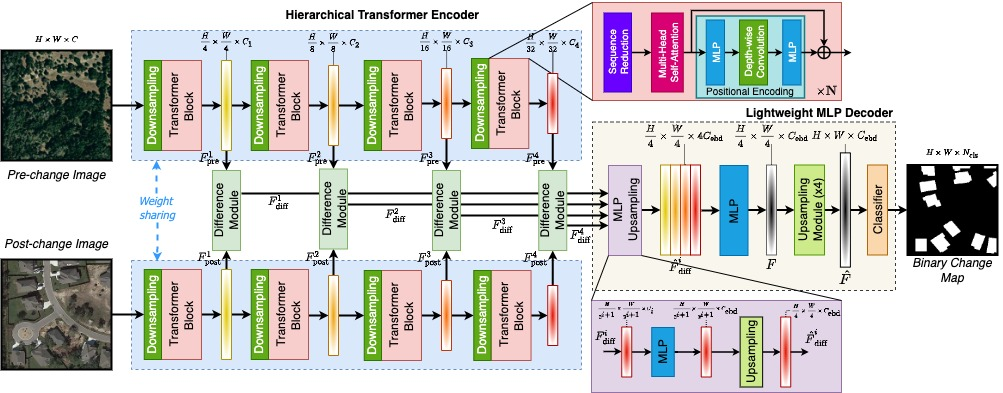
\includegraphics[width=\textwidth]{images/IGARS_ChangeFormer.jpeg}
    \caption{Overview of the baseline ChangeFormer architecture. Recovery from ChangeFormer original paper \cite{Bandara2022ChangeFormer}}
    \label{fig:changeformer_architecture}
\end{figure*}


\noindent \textbf{Efficient and Linear Attention Mechanisms}.  
To mitigate the quadratic cost of MHSA \cite{Vaswani2017Attention}, several efficient attention mechanisms have been proposed. Kernelized linear attention methods, including the Performer \cite{Choromanski2021Performer} and Linear Transformers \cite{Katharopoulos2020Linear}, replace softmax attention with feature maps to achieve $\mathcal{O}(N)$ complexity. Low–rank approximations such as Linformer \cite{Wang2020Linformer} and Nyströmformer \cite{Xiong2021Nystromformer} reduce computation by projecting the attention matrix into lower–dimensional spaces. Windowed or sparse variants (e.g., Swin Transformer \cite{Liu2021Swin} and Sparsifiner \cite{Wei2023Sparsifiner}) restrict token interactions to learned or structured neighborhoods. Although effective in some vision tasks, these approaches often suffer from reduced feature diversity due to inherent low–rank behavior, which limits performance in dense prediction tasks such as semantic segmentation. Rank–Augmented Linear Attention (RALA) \cite{Fan2025RALA} directly addresses this issue by increasing the rank of the key–value representation through token–wise weighting and output modulation.

\noindent \textbf{Gap in the Literature}.  
Despite progress in both BCD architectures and efficient attention mechanisms, rank–augmented linear attention has not been explored in multi–temporal remote sensing. Existing BCD Transformers still depend on full MHSA \cite{Vaswani2017Attention}, which constrains scalability to high resolutions and limits feasible batch sizes. Likewise, prior efficient attention techniques have not been systematically evaluated under the spatial–temporal constraints of bi–temporal BCD. This motivates the integration of RALA into a BCD architecture to improve efficiency while maintaining segmentation accuracy.
\section{\uppercase{Theoretical Background}}
\label{sec:theoretical}

This section presents the proposed \textbf{RALA-ChangeFormer}, a computationally efficient variant of ChangeFormer in which the quadratic Multi-Head Self-Attention (MHSA) is replaced with rank-augmented linear attention (RALA). In order to provide a better understanding, we organized the paragraphs: (i) a brief overview of ChangeFormer, (ii) a clear formulation of Rank-Augmented Linear Attention (RALA), and (iii) the integration into the bi-temporal encoder–decoder design. In addition, this section introduces the theoretical formulation that underpins the proposed method, providing the mathematical foundations required for its implementation and analysis.

\subsection{ChangeFormer}
\label{subsec:cf_overview}

ChangeFormer~\cite{Bandara2022ChangeFormer} is a hierarchical Siamese encoder-decoder architecture designed for bi-temporal building change detection. An overview of the full architecture is shown in Fig.~\ref{fig:changeformer_architecture}. Given two VHR images 
$I_{t_1}$ and $I_{t_2}$, the model processes them through a shared convolutional encoder to obtain multi-scale feature maps
\begin{equation}
F_{t_1}^{(l)},\, F_{t_2}^{(l)} \in \mathbb{R}^{H_l \times W_l \times C_l},
\end{equation}
where $l$ denotes the resolution level in the hierarchy. The encoder follows the same design principle as hierarchical Vision Transformer backbones such as Swin~\cite{Teng2023SwinCD}: the spatial resolution is progressively reduced while channel dimensionality increases, enabling the model to capture both fine-grained local texture and broader semantic context across scales.

At each scale, the bi-temporal feature maps are concatenated channel-wise and projected into a sequence of tokens via a lightweight patch embedding module:
\begin{equation}
X^{(l)} = \mathrm{PatchEmbed}\!\left(F_{t_1}^{(l)} \,\Vert\, F_{t_2}^{(l)}\right)
      \in \mathbb{R}^{N_l \times C_l},
\end{equation}
where $N_l = H_lW_l$ is the number of tokens at level $l$.

The decoder is composed of a cascade of Transformer blocks operating at multiple resolutions. Each block contains Multi-Head Self-Attention (MHSA) and a feed-forward network (FFN), refining token representations through long-range spatio-temporal interactions before upsampling and fusion into the final change mask.

Because MHSA has quadratic complexity in the sequence length ($\mathcal{O}(N_l^2)$), the decoder becomes the dominant computational bottleneck for VHR imagery where $N_l$ is large. Furthermore, this architecture does not incorporate the shifted-window mechanism used in Swin Transformer~\cite{Teng2023SwinCD}, which further limits its ability to efficiently capture long-range dependencies at lower computational cost. This motivates the integration of a more efficient attention mechanism—specifically, rank-augmented linear attention—to reduce computational cost while preserving the representational capacity required for accurate change detection.


\subsection{Rank-Augmented Linear Attention}
\label{subsec:rala}

Linear attention methods aim to reduce the $\mathcal{O}(N^2)$ cost of standard softmax attention by replacing the kernel with a feature map $\kappa(\cdot)$. Standard attention is defined as
\begin{equation}
\mathrm{Attn}(Q,K,V)=\mathrm{softmax}\!\left(\frac{QK^\top}{\sqrt{d}}\right)V,
\label{eq:softmax_attention}
\end{equation}
where $Q,K,V\in\mathbb{R}^{N\times d}$ \cite{Vaswani2017Attention} contain the queries, keys, and values for the $N$ input tokens (each row $Q_i$ is the query vector of token $i$), and $d$ denotes the hidden embedding dimension. Forming the dense matrix $QK^\top$ produces quadratic time and memory cost.

Linear attention replaces the softmax kernel with a feature map:
\begin{equation}
\mathrm{Attn}_{\text{lin}}(Q,K,V)=\kappa(Q)\big(\kappa(K)^\top V\big),
\label{eq:linear_attention}
\end{equation}
where $\mathcal{\kappa(.)}$ is a kernel feature map, reducing the complexity to $\mathcal{O}(Nd)$.  
The intermediate matrix
\begin{equation}
\kappa(K)^\top V \in\mathbb{R}^{d\times d}
\label{eq:B_def}
\end{equation}
acts as a global key–value aggregation buffer. In practice, the equation \ref{eq:B_def} often becomes \emph{low-rank} because many key vectors are nearly collinear. This collapse in feature diversity limits representational power and degrades dense prediction performance.

\paragraph{Rank Augmentation.}
RALA~\cite{Fan2025RALA} addresses this by explicitly increasing the rank of $B$. Let $K_j$ and $V_j$ denote the key and value vectors of token $j$. RALA constructs
\begin{equation}
B=\sum_{j=1}^{N}\alpha_j\,\kappa(K_j)^\top V_j ,
\label{eq:rala_rank_aug}
\end{equation}

\begin{equation}
N=\sum_{j=1}^{N}\alpha_j
\label{eq:rala_alpha_aug}
\end{equation}

\noindent where $\alpha_j$ reweights each token using a \emph{global query vector}
\begin{equation}
Q_{\mathrm{g}}=\frac{1}{N}\sum_{i=1}^N Q_i,
\label{eq:global_query}
\end{equation}
encoding the overall semantic content of the sequence. The weights are computed as
\begin{equation}
\alpha_j=N \times \frac{\exp(Q_{\mathrm{g}}\kappa(K_j)^\top)}
{\sum_{m=1}^{N}\exp(Q_{\mathrm{g}}\kappa(K_m)^\top)},
\label{eq:alpha_softmax}
\end{equation}
which emphasizes information-rich tokens and increases the effective rank of $B$.

\paragraph{Output Feature Modulation.}
Even if $B$ achieves a full-rank state, the output features
\begin{equation}
Y_i=\kappa(Q_i)\,B
\label{eq:Y_pre_modulation}
\end{equation}
may still be low-rank.  
This follows from the matrix inequality
\begin{equation}
\mathrm{Rank}(Y)\le \min\big(\mathrm{Rank}(\kappa(Q)),\,\mathrm{Rank}(B)\big)\le d,
\label{eq:rank_inequality}
\end{equation}
which states that the output cannot have rank greater than its limiting factors: the diversity of queries \(\kappa(Q)\) and the diversity of the aggregated buffer \(B\). When $\kappa$ contains many correlated query vectors (common in remote sensing patches), $\mathrm{Rank}(\kappa(Q))<d$, causing information loss even if $B$ is full-rank.

To restore feature diversity, RALA introduces a token-wise modulation step:
\begin{equation}
Y_i=\phi(X_i)\odot \Big(\kappa(Q_i)\,B\Big),
\label{eq:Yi_modulated}
\end{equation}
where $\phi(\cdot)$ is a token-dependent transform applied only for modulation, and $\odot$ denotes the Hadamard product.  
This injects token-specific information without increasing the asymptotic cost and increases the expressive rank of the output.
This operation injects token-specific information into the output features, complementing the global mixing performed by $B$ and effectively increasing the expressive rank of $Y$. The modulation is applied only channel-wise, preserving the linear-time complexity of the attention operation.

\begin{figure}[t]
    \centering
    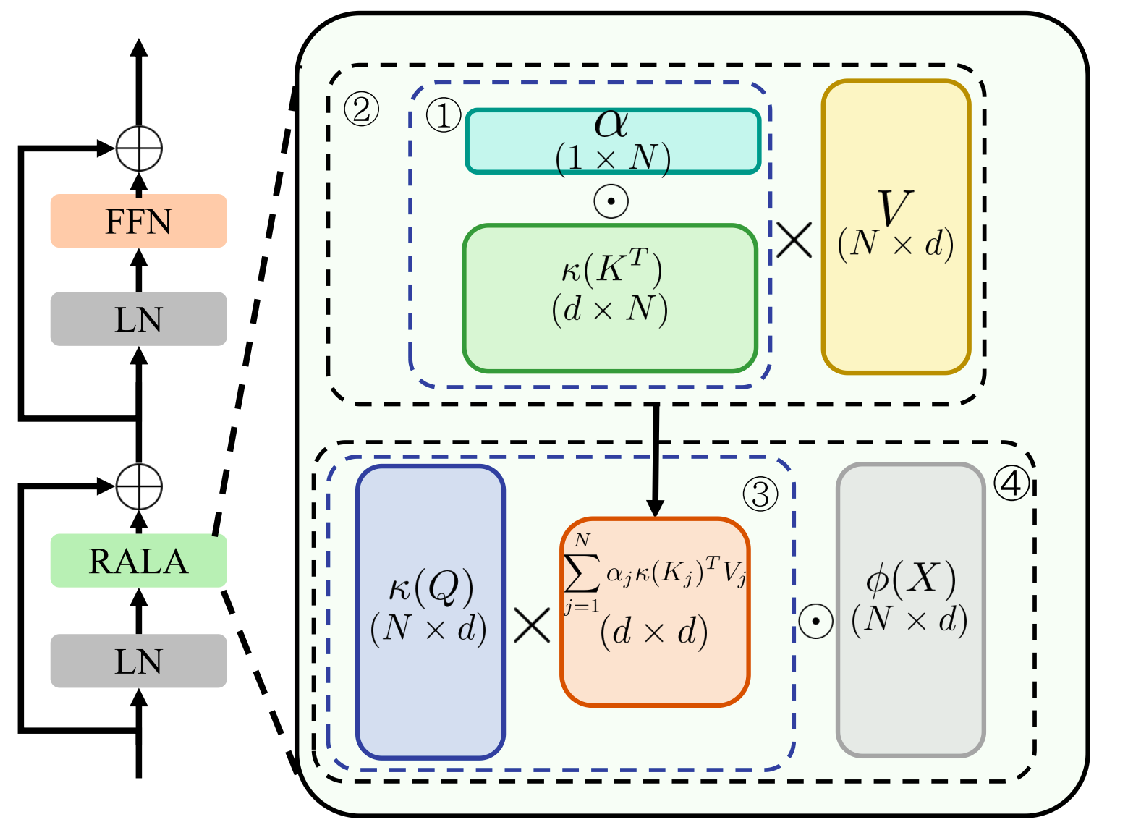
\includegraphics[width=\linewidth]{images/RALA.png}
    \caption{RALA Transformer block replacing the standard MHSA module. Recovery from RALA original paper \cite{Fan2025RALA}}
    \label{fig:rala_block}
\end{figure}
\section{\uppercase{Method}}
\label{sec:method}

RALA-ChangeFormer is constructed by replacing every MHSA block in the \textbf{encoder} of ChangeFormer with the rank-augmented linear attention module described in Section~\ref{subsec:rala}, where attention-related computational costs are dominant. All remaining components-CNN encoder, feed-forward layers, skip connections, and multi-scale fusion-remain unchanged, preserving full architectural compatibility with the baseline design. The integration mechanism is summarized in Figure~\ref{fig:rala_block}.

Given the token sequence $X^{(l)} \in \mathbb{R}^{N_l \times C_l}$ at resolution level $l$, the block first computes query, key, and value projections
\begin{equation}
Q = X^{(l)}W_Q,\qquad
K = X^{(l)}W_K,\qquad
V = X^{(l)}W_V,
\label{eq:qkv_projection}
\end{equation}

after which the attention operation proceeds exactly following the equations introduced in Section~\ref{subsec:rala}, namely: the global query descriptor (Eq.~\ref{eq:global_query}), the token-wise relevance coefficients (Eq.~\ref{eq:alpha_softmax}), the rank-augmented key–value buffer (Eq.~\ref{eq:rala_rank_aug}), and the modulated output features (Eq.~\ref{eq:Yi_modulated}).

The resulting token-specific attention output $A$ replaces the MHSA output of the original ChangeFormer block and is incorporated via a residual connection:
\begin{equation}
X_{\text{out}}
    = X^{(l)} + \mathrm{LN}(A),
\qquad
Y = \mathrm{FFN}(X_{\text{out}}),
\label{eq:residual_ffn}
\end{equation}

This construction preserves the overall representational structure of the original ChangeFormer architecture-including multi-scale refinement, long-range reasoning, and residual learning-while substituting the quadratic-cost MHSA blocks \textbf{exclusively within the encoder} with a linear-time rank-augmented mechanism.

\noindent\textbf{Computational Complexity.}
Let $N$ denote the number of tokens and $d$ the hidden dimension.  
Standard MHSA requires \textbf{time: }$\mathcal{O}(N^{2}d)$ and \textbf{memory: }$\mathcal{O}(N^{2})$ due to the formation of the dense $N\times N$ attention matrix.  
In contrast, the RALA module scales as \textbf{time: }$\mathcal{O}(Nd)$ and \textbf{memory: }$\mathcal{O}(d^{2})$ because no pairwise token interactions are constructed explicitly.  
Since $N \gg d$ for VHR remote sensing images, this substitution results in substantially reduced computational cost and enables significantly larger batch sizes, faster training, and improved scalability to higher spatial resolutions.

Functionally, the architecture preserves all capabilities of ChangeFormer—multi-scale feature reasoning, long-range spatial interactions, and precise boundary refinement—while reducing the computational burden within each Transformer block. Because RALA operates as a drop-in replacement for MHSA, the model maintains full compatibility with pretraining strategies, multi-scale inference, and existing training pipelines. This makes RALA-ChangeFormer suitable for high-resolution BCD and scalable to large bi-temporal datasets under fixed GPU budgets.
\section{\uppercase{Experiments and Results}}
\label{sec:experiments}

\noindent
In order to show the effectiveness of RALA-ChangeFormer, we evaluate our proposal on two widely used benchmarks. Our experiments assess both segmentation accuracy and computational efficiency after replacing the quadratic MHSA modules of ChangeFormer with the RALA mechanism. All comparisons are made against the original ChangeFormer \cite{Bandara2022ChangeFormer}.

\noindent \textbf{LEVIR-CD.} LEVIR-CD \cite{Zheng2020LEVIR} contains 637 bi-temporal high-resolution image pairs (1024$\times$1024) depicting building changes in rapidly developing urban areas. Following standard practice, each pair is cropped into non-overlapping 256$\times$256 tiles, yielding: \text{Train/Val/Test} = 6096 / 762 / 762.

\noindent \textbf{DSIFN-CD.} DSIFN-CD \cite{Shen2021DSIFN} includes multi-class land-cover and building change scenes under heterogeneous imaging conditions. Each 512$\times$512 pair is divided into non-overlapping 256$\times$256 tiles, producing: \text{Train/Val/Test} = 14400 / 1360 / 192.

Ground-truth labels in both datasets are binary change masks. For efficiency experiments, the following is added (i) input patch resolution, and (ii) batch size until GPU out-of-memory (OOM) is reached.

\noindent \textbf{Implementation Details.} All experiments are implemented in PyTorch, matching the software environment used by the ChangeFormer implementation \cite{Bandara2022ChangeFormer} for fair comparison.

For \textbf{LEVIR-CD}, both ChangeFormer (CF) and RALA-ChangeFormer (RALA-CF) are initialized from the SegFormer-B2 encoder pretrained on ADE20K, following the training protocol of the original ChangeFormer~\cite{Bandara2022ChangeFormer}. An initial learning rate with cosine decay of $1\times10^{-4}$ is used.

For \textbf{DSIFN-CD}, CF is fine-tuned from the best CF checkpoint obtained on LEVIR-CD using a reduced learning rate of $6\times10^{-5}$. Analogously, RALA-CF is initialized from the best RALA-CF checkpoint trained on LEVIR-CD and optimized under the same schedule. In all experiments, the only architectural difference between CF and RALA-CF lies in the encoder attention modules (standard MHSA vs.\ rank-augmented linear attention).


\subsection{Evaluation Metrics}

We report standard change detection metrics following the state-of-the-art BCD models \cite{Zheng2020LEVIR, Shen2021DSIFN, Bandara2022ChangeFormer, Chen2022BIT, Fang2021SNUNetCD}. To measure computational efficiency, we additionally track (a) total learnable parameters, (b) GFLOPs per forward pass, (c) peak GPU memory consumption, (d) maximum feasible batch size before OOM and (e) training throughput (images/s).

\noindent \textbf{Results on Segmentation Accuracy}

\begin{table}[h!]
\caption{Segmentation accuracy of baseline BCD models and our variants on LEVIR-CD and DSIFN-CD using $256\times256$ input patches and batch size 16. 
Metrics for SNUNet-CD and BIT are taken from the original ChangeFormer paper \cite{Bandara2022ChangeFormer}.}
\label{tab:accuracy}
\centering
\resizebox{\columnwidth}{!}{
\begin{tabular}{lcccc}
\hline
\textbf{Model} & \textbf{Dataset} & \textbf{F1} & \textbf{IoU} & \textbf{OA} \\
\hline
SNUNet-CD~\cite{Fang2021SNUNetCD} & LEVIR-CD & 88.16 & 78.83 & 98.82 \\
BIT~\cite{Chen2022BIT}            & LEVIR-CD & 89.31 & 80.68 & 98.92 \\
CF~\cite{Bandara2022ChangeFormer} & LEVIR-CD & 90.40 & 82.48 & 99.04 \\
\rowcolor{pastelorange}
RALA-CF (ours) & LEVIR-CD & \textbf{89.87} & \textbf{81.60} & \textbf{98.99} \\

\hline
SNUNet-CD~\cite{Fang2021SNUNetCD} & DSIFN-CD & 66.18 & 49.45 & 87.34 \\
BIT~\cite{Chen2022BIT}            & DSIFN-CD & 69.26 & 52.97 & 89.41 \\
CF~\cite{Bandara2022ChangeFormer} & DSIFN-CD & 86.67 & 76.48 & 95.56 \\
\rowcolor{pastelorange}
RALA-CF (ours) & DSIFN-CD & \textbf{84.07} & \textbf{73.96} & \textbf{92.44} \\
\hline
\end{tabular}
}
\end{table}

\noindent As shown in Table~\ref{tab:accuracy}, RALA-CF matches the segmentation accuracy of the baseline ChangeFormer on both datasets, while outperforming prior BCD models such as BIT and SNUNet-CD. This indicates that replacing MHSA with rank-augmented linear attention preserves the segmentation capability of ChangeFormer.

\noindent \textbf{Efficiency Analysis}.

\begin{table}[h!]
\caption{Efficiency comparison between ChangeFormer and RALA-ChangeFormer ($256\times256$ inputs, batch size 16).}
\label{tab:efficiency}
\centering
\resizebox{\columnwidth}{!}{
\begin{tabular}{lccc}
\hline
\textbf{Model} & \textbf{Params (M)} & \textbf{GFLOPs} & \textbf{Peak VRAM (GB)} \\
\hline
CF & 247 & 248.77 & 27 \\
\rowcolor{pastelorange}
RALA-CF & \textbf{243} & \textbf{228.62} & \textbf{21} \\
\hline
\end{tabular}
}
\end{table}

\noindent Table~\ref{tab:efficiency} shows that RALA-CF reduces FLOPs by approximately 8--10\% and peak memory usage by \textbf{20--30}\% without altering the overall architecture. These savings translate into faster training and more flexible batch-size configurations.

\noindent \textbf{Maximum Batch Size Experiments}

\begin{table}[h!]
\caption{Maximum batch size before OOM for different input resolutions. VRAM limit: 34--36 GB (A100 40 GB VRAM GPU).}
\label{tab:batch_multires}
\centering
\resizebox{\columnwidth}{!}{
\begin{tabular}{lccc}
\hline
\textbf{Resolution} & \textbf{Model} & \textbf{Max Batch} & \textbf{VRAM at OOM (GB)} \\
\hline
\multirow{256$\times$256} 
& CF       & 32 & 34 \\
& RALA-CF  & \textbf{48} & \textbf{34} \\
\hline
\multirow{512$\times$512} 
& CF       & 8  & 34 \\
& RALA-CF  & \textbf{12} & \textbf{34} \\
\hline
\multirow{1024$\times$1024} 
& CF       & 2  & 36 \\
& RALA-CF  & \textbf{3} & \textbf{36} \\
\hline
\end{tabular}
}
\end{table}

\noindent \textbf{Ablation: MHSA vs.\ RALA}. To isolate the contribution, we perform an ablation where only encoder attention is replaced with RALA, and all other components remain unchanged.

\begin{table}[h!]
\caption{Ablation study isolating the encoder attention mechanism.}
\label{tab:ablation}
\centering
\resizebox{\columnwidth}{!}{
\begin{tabular}{lccc}
\hline
\textbf{Variant} & \textbf{GFLOPs} & \textbf{VRAM (GB)} \\
\hline
Baseline MHSA & 86.17 & 12 \\
\rowcolor{pastelorange}
Encoder: RALA & \textbf{76.95} & \textbf{8} \\
\hline
\end{tabular}
}
\end{table}

\noindent As shown in Table~\ref{tab:ablation}, most computational savings originate from replacing MHSA within the encoder, where token counts are highest and attention cost dominates.

\subsection{Discussion}
\label{sec:discussion}

The experimental results demonstrate that integrating RALA into the encoder of ChangeFormer provides consistent computational advantages while preserving segmentation accuracy in multi-temporal BCD. Since the modification affects only the encoder self-attention modules—leaving the convolutional backbone, FFN layers, and decoder head unchanged—the magnitude of improvements is moderate but systematic across all benchmarks.

\noindent \textbf{Accuracy–Efficiency Balance.}
As shown in Table~\ref{tab:accuracy}, RALA-ChangeFormer achieves nearly identical F1, IoU, and OA scores to the baseline ChangeFormer on both datasets \cite{Zheng2020LEVIR,Shen2021DSIFN}. The differences fall within normal training variance, indicating that the rank-augmented linear formulation retains the model’s ability to represent spatial–temporal interactions between bi-temporal features maps. Importantly, while many linear-attention variants \cite{Choromanski2021Performer,Wang2020Linformer,Xiong2021Nystromformer} exhibit a well-documented degradation in dense vision problems due to low-rank collapse, RALA avoids this issue by explicitly increasing the diversity of its KV buffer. This preservation of representational capacity is further illustrated by the attention maps in Fig.~\ref{fig:attn_maps}, which provide a qualitative visualization of the spatial attention distribution. Collectively, these results confirm that RALA maintains reliable prediction for this specific tasks, despite replacing quadratic attention.

\noindent \textbf{Computational Benefits and Practical Scalability.}
Table~\ref{tab:efficiency} shows clear reductions in FLOPs and peak VRAM usage when MHSA is replaced with RALA. Although iteration-level speedups are modest, the improvements compound at higher resolutions, where MHSA cost is highest. The increased feasible batch sizes (Table~\ref{tab:batch_multires}) highlight the most practical advantage: RALA-CF can process substantially more images per iteration under identical hardware constraints. In the context of remote sensing, where datasets may contain tens or hundreds of thousands of patches, this translates into significantly higher throughput and faster experimentation cycles. Moreover, training with larger batches allows exposure to more diverse samples per step, improving stability and enabling efficient learning on large, out-of-distribution datasets. In contrast, baseline MHSA-based architectures often require prohibitively small batches that impair convergence behavior on heterogeneous datasets such as DSIFN-CD.

\noindent \textbf{Encoder-Level Efficiency Gains.}
The ablation in Table~\ref{tab:ablation} isolates the source of the computational savings, showing that almost all reductions originate from the encoder, where token density is highest and attention cost dominates. The decoder contributes marginally to computational load, so modifying only the encoder yields the majority of benefits while maintaining full architecture compatibility.

In summary, RALA-ChangeFormer achieves meaningful efficiency gains without compromising segmentation quality, while offering practical scalability advantages for high-resolution or large-scale BCD pipelines under fixed GPU memory budgets.

\begin{figure}[t]
    \centering
    \begin{subfigure}{0.48\linewidth}
        \centering
        
\includegraphics[width=\linewidth]{images/Attention_Map_CF.pdf}
        \caption{CF (MHSA).}
        \label{fig:attn_cf}
    \end{subfigure}
    \hfill
    \begin{subfigure}{0.48\linewidth}
        \centering
        
\includegraphics[width=\linewidth]{images/Attention_Map_RALA_CF.pdf}
        \caption{RALA-CF (RALA).}
        \label{fig:attn_rala}
    \end{subfigure}
    \caption{Token-wise attention maps at the last encoder stage
    ($N{=}512$ tokens on the x-axis, $d{=}64$ channels on the y-axis) for the baseline ChangeFormer and the proposed RALA-ChangeFormer.
    Colors represent normalized attention intensity, where darker values indicate low attention response and brighter (purple) values indicate higher attention. The maps are shown for qualitative comparison only, illustrating that RALA preserves non-collapsing spatial attention patterns comparable to MHSA.}
    \label{fig:attn_maps}
\end{figure}

\subsection{Limitations}
\label{subsec:limitations}

Despite the advantages demonstrated in Sections~\ref{sec:experiments} and~\ref{sec:discussion}, the proposed integration of rank-augmented linear attention exhibits several limitations that contextualize its practical impact.

\noindent \textbf{(1) Moderate end-to-end computational gains.} Although rank augmentation substantially reduces the cost of encoder self-attention, the overall computational footprint of ChangeFormer is still influenced by multiscale fusion layers. As shown in Table~\ref{tab:efficiency}, the reduction in total GFLOPs remains moderate (8--10\%), since attention constitutes only part of the complete pipeline.


\noindent \textbf{(2) Efficiency improvements grow with token count.} RALA provides the largest benefits when the number of tokens is high (e.g., 512 or 1024 resolution). At lower input sizes such as $256\times256$, improvements are measurable but less pronounced, which limits impact for applications operating strictly at small patch resolutions.

\noindent \textbf{(3) Limited impact on model expressiveness beyond attention.} While RALA mitigates the low-rank collapse common in linear attention and preserves segmentation performance, it does not enhance the expressive capacity of non-attention modules such as convolutional encoders or decoder fusion layers. As a result, the overall accuracy remains bounded by the representational capacity of the original ChangeFormer architecture.

\noindent \textbf{(4) Limited evaluation on independent acquisition domains.}
The experimental evaluation follows the standard training and testing protocols of LEVIR-CD and DSIFN-CD, where splits are spatially disjoint but not fully independent in terms of acquisition conditions or geographic regions. While this work focuses on computational scalability and efficiency under commonly adopted BCD benchmarks, the generalization of RALA-ChangeFormer to unseen acquisition domains (e.g., cross-region or cross-sensor settings) remains an open question. Evaluating rank-augmented linear attention under fully independent data distributions is a promising direction for future work.

\medskip
\noindent  Overall, although the proposed integration offers practical advantages in memory efficiency, scalability, and batch-size flexibility, it does not eliminate the structural constraints inherent to hierarchical encoder--decoder architectures. These considerations frame the scope of improvements achieved by substituting MHSA with rank-augmented linear attention.

\section{\uppercase{Conclusion}} 
\label{sec:conclusion}

This work introduced \textbf{RALA-ChangeFormer}, an efficient variant of ChangeFormer in which the multi-head self-attention modules of the \textbf{encoder} are replaced with rank-augmented linear attention. All remaining components of the architecture, including the convolutional backbone, feed-forward layers, and the lightweight MLP decoder, remain unchanged. The goal of this modification is to alleviate the quadratic cost of MHSA in high-token regimes while preserving the representational capacity required for multi-temporal building change detection.

Experimental evaluations on LEVIR-CD and DSIFN-CD show that RALA-ChangeFormer maintains segmentation accuracy comparable to the baseline model, confirming that the rank-augmented KV buffer is sufficiently expressive for bi-temporal spatial-temporal reasoning. Importantly, unlike previous linear-attention formulations, RALA avoids the low-rank collapse typically observed in dense prediction tasks, as further illustrated by the qualitative attention-map comparisons.

From a computational perspective, the proposed encoder-level integration yields consistent reductions in attention-related FLOPs and peak GPU memory usage, and increases feasible batch sizes, particularly at higher resolutions where attention costs dominate. These improvements enhance practical scalability under fixed memory budgets, enabling the model to process more patches per iteration and to support efficient training in high-resolution or large-batch settings without increasing hardware requirements. Overall, the results demonstrate that RALA-ChangeFormer provides a favorable accuracy-efficiency trade-off for VHR change detection, preserving predictive behaviour while reducing resource demands.

Rather than proposing a novel change detection formulation, this work aims to empirically assess whether modern linear-attention mechanisms can be integrated into hierarchical bi-temporal change detection architectures without degrading performance, and to quantify the resulting efficiency-accuracy trade-offs. In this context, several promising directions remain for future work. One avenue is to explore adaptive or data-dependent strategies that refine the rank selection in RALA, potentially drawing on matrix reconstruction techniques such as SVD to further enhance representational diversity. Another promising direction is the integration of RALA into multi-scale or multi-task BCD frameworks, enabling a more robust evaluation of its generalization capacity across heterogeneous settings. Finally, with generative approaches—such as diffusion and flow-matching models—emerging as powerful alternatives for BCD, a key opportunity lies in developing memory-efficient attention formulations that can be embedded into these computationally demanding architectures.


\section*{\uppercase{Acknowledgements}}

We gratefully acknowledge the support of the GINIA research group, where this work was initiated. GINIA provided an academic research environment that supported the early stages of this work in urban data analysis and covered the conference registration fee.

%\textit{$\backslash$section*\{ACKNOWLEDGEMENTS\}}

\bibliographystyle{IEEEtran}
{\small
\bibliography{example}}

\end{document}